% Graphic for TeX using PGF
% Title: /home/biensuanga/Documents/Projet/gk/Realisation/Diagramme1.dia
% Creator: Dia v0.97.2
% CreationDate: Thu Mar 13 15:45:37 2014
% For: biensuanga
% \usepackage{tikz}
% The following commands are not supported in PSTricks at present
% We define them conditionally, so when they are implemented,
% this pgf file will use them.
\ifx\du\undefined
  \newlength{\du}
\fi
\setlength{\du}{15\unitlength}
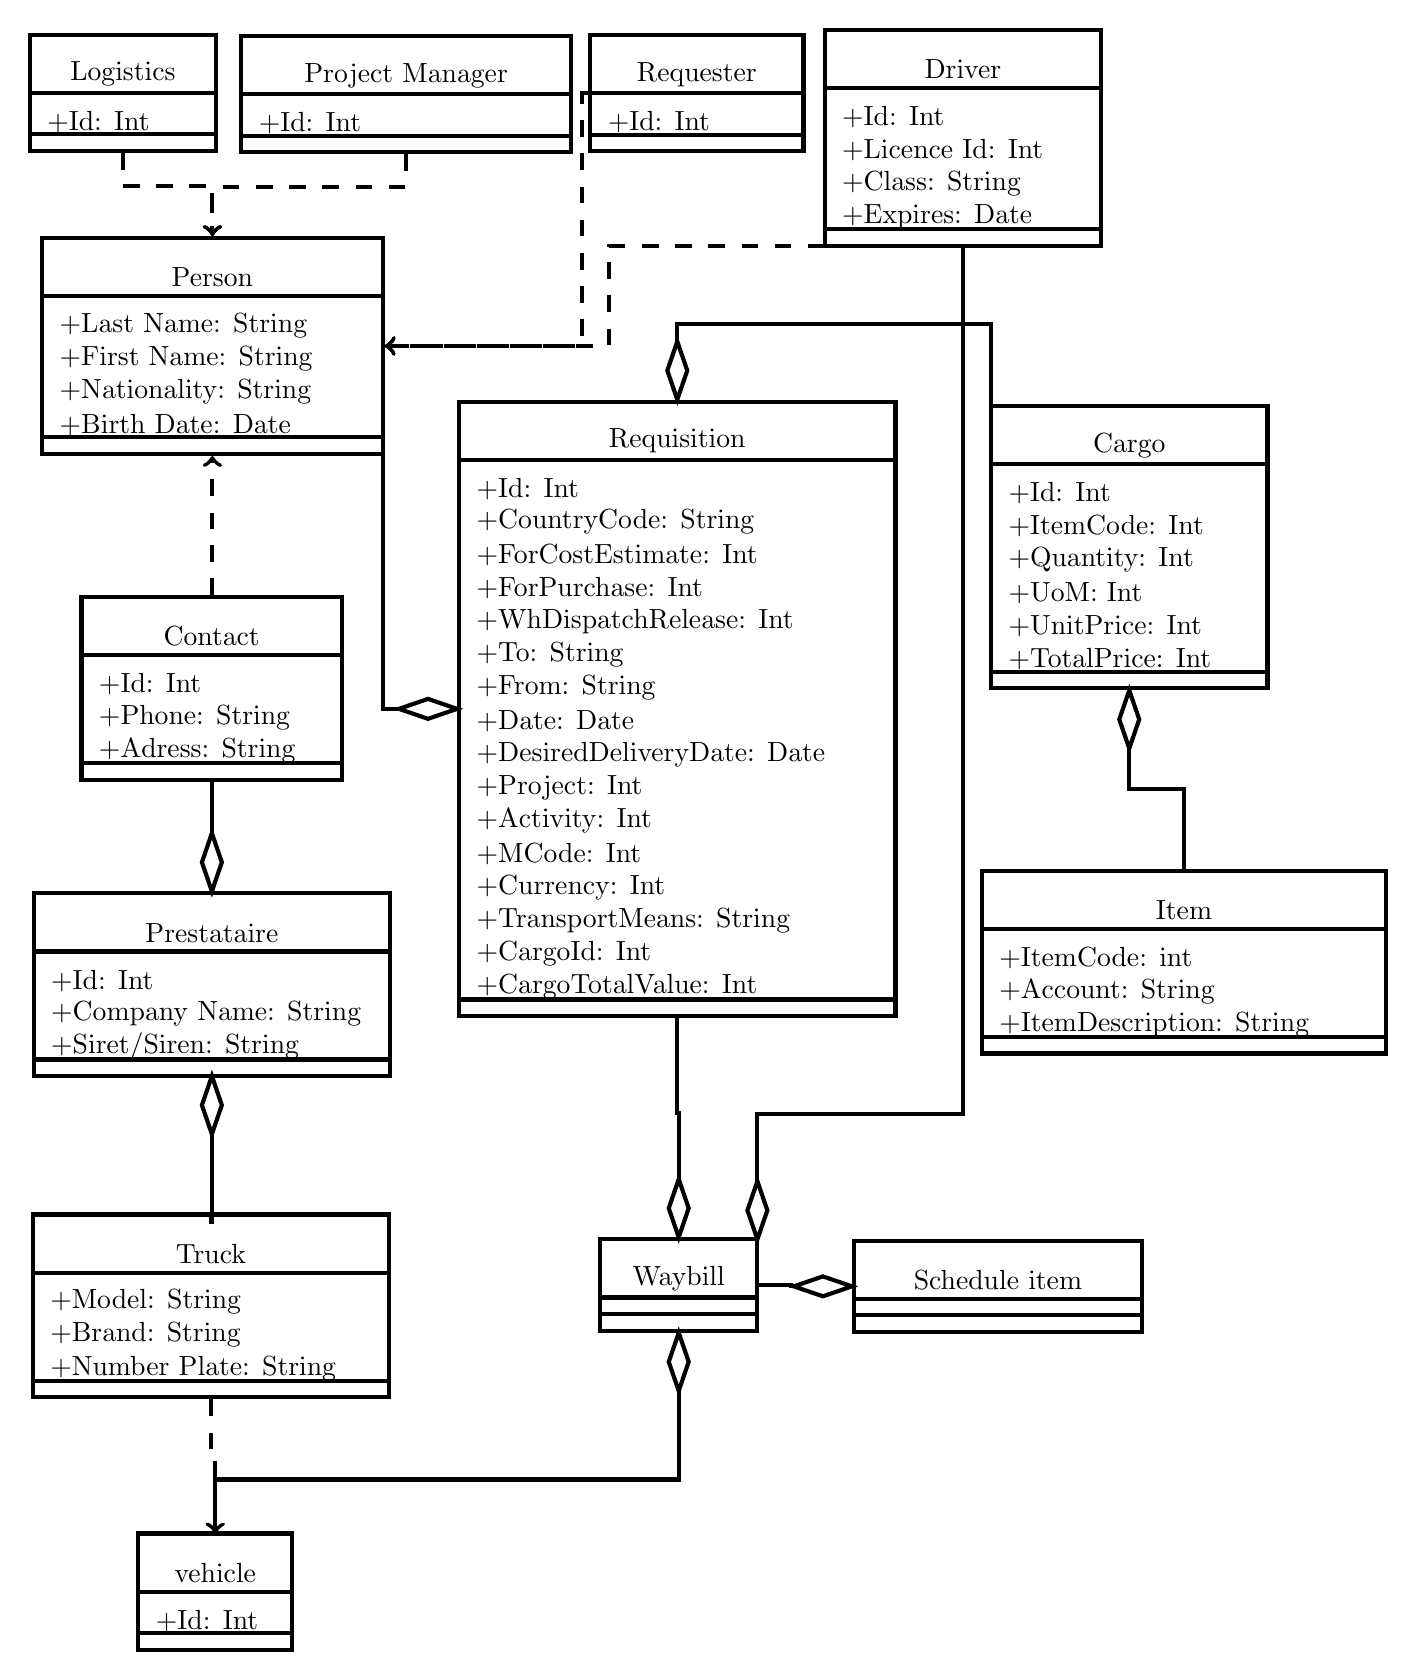
\begin{tikzpicture}
\pgftransformxscale{1.000000}
\pgftransformyscale{-1.000000}
\definecolor{dialinecolor}{rgb}{0.000000, 0.000000, 0.000000}
\pgfsetstrokecolor{dialinecolor}
\definecolor{dialinecolor}{rgb}{1.000000, 1.000000, 1.000000}
\pgfsetfillcolor{dialinecolor}
\pgfsetlinewidth{0.100000\du}
\pgfsetdash{}{0pt}
\definecolor{dialinecolor}{rgb}{1.000000, 1.000000, 1.000000}
\pgfsetfillcolor{dialinecolor}
\fill (0.627412\du,4.970010\du)--(0.627412\du,6.370010\du)--(8.827412\du,6.370010\du)--(8.827412\du,4.970010\du)--cycle;
\definecolor{dialinecolor}{rgb}{0.000000, 0.000000, 0.000000}
\pgfsetstrokecolor{dialinecolor}
\draw (0.627412\du,4.970010\du)--(0.627412\du,6.370010\du)--(8.827412\du,6.370010\du)--(8.827412\du,4.970010\du)--cycle;
% setfont left to latex
\definecolor{dialinecolor}{rgb}{0.000000, 0.000000, 0.000000}
\pgfsetstrokecolor{dialinecolor}
\node at (4.727412\du,5.920010\du){Person};
\definecolor{dialinecolor}{rgb}{1.000000, 1.000000, 1.000000}
\pgfsetfillcolor{dialinecolor}
\fill (0.627412\du,6.370010\du)--(0.627412\du,9.770010\du)--(8.827412\du,9.770010\du)--(8.827412\du,6.370010\du)--cycle;
\definecolor{dialinecolor}{rgb}{0.000000, 0.000000, 0.000000}
\pgfsetstrokecolor{dialinecolor}
\draw (0.627412\du,6.370010\du)--(0.627412\du,9.770010\du)--(8.827412\du,9.770010\du)--(8.827412\du,6.370010\du)--cycle;
% setfont left to latex
\definecolor{dialinecolor}{rgb}{0.000000, 0.000000, 0.000000}
\pgfsetstrokecolor{dialinecolor}
\node[anchor=west] at (0.777412\du,7.070010\du){+Last Name: String};
% setfont left to latex
\definecolor{dialinecolor}{rgb}{0.000000, 0.000000, 0.000000}
\pgfsetstrokecolor{dialinecolor}
\node[anchor=west] at (0.777412\du,7.870010\du){+First Name: String};
% setfont left to latex
\definecolor{dialinecolor}{rgb}{0.000000, 0.000000, 0.000000}
\pgfsetstrokecolor{dialinecolor}
\node[anchor=west] at (0.777412\du,8.670010\du){+Nationality: String};
% setfont left to latex
\definecolor{dialinecolor}{rgb}{0.000000, 0.000000, 0.000000}
\pgfsetstrokecolor{dialinecolor}
\node[anchor=west] at (0.777412\du,9.470010\du){+Birth Date: Date};
\definecolor{dialinecolor}{rgb}{1.000000, 1.000000, 1.000000}
\pgfsetfillcolor{dialinecolor}
\fill (0.627412\du,9.770010\du)--(0.627412\du,10.170010\du)--(8.827412\du,10.170010\du)--(8.827412\du,9.770010\du)--cycle;
\definecolor{dialinecolor}{rgb}{0.000000, 0.000000, 0.000000}
\pgfsetstrokecolor{dialinecolor}
\draw (0.627412\du,9.770010\du)--(0.627412\du,10.170010\du)--(8.827412\du,10.170010\du)--(8.827412\du,9.770010\du)--cycle;
\pgfsetlinewidth{0.100000\du}
\pgfsetdash{}{0pt}
\definecolor{dialinecolor}{rgb}{1.000000, 1.000000, 1.000000}
\pgfsetfillcolor{dialinecolor}
\fill (19.476200\du,-0.048711\du)--(19.476200\du,1.351289\du)--(26.136200\du,1.351289\du)--(26.136200\du,-0.048711\du)--cycle;
\definecolor{dialinecolor}{rgb}{0.000000, 0.000000, 0.000000}
\pgfsetstrokecolor{dialinecolor}
\draw (19.476200\du,-0.048711\du)--(19.476200\du,1.351289\du)--(26.136200\du,1.351289\du)--(26.136200\du,-0.048711\du)--cycle;
% setfont left to latex
\definecolor{dialinecolor}{rgb}{0.000000, 0.000000, 0.000000}
\pgfsetstrokecolor{dialinecolor}
\node at (22.806200\du,0.901289\du){Driver};
\definecolor{dialinecolor}{rgb}{1.000000, 1.000000, 1.000000}
\pgfsetfillcolor{dialinecolor}
\fill (19.476200\du,1.351289\du)--(19.476200\du,4.751289\du)--(26.136200\du,4.751289\du)--(26.136200\du,1.351289\du)--cycle;
\definecolor{dialinecolor}{rgb}{0.000000, 0.000000, 0.000000}
\pgfsetstrokecolor{dialinecolor}
\draw (19.476200\du,1.351289\du)--(19.476200\du,4.751289\du)--(26.136200\du,4.751289\du)--(26.136200\du,1.351289\du)--cycle;
% setfont left to latex
\definecolor{dialinecolor}{rgb}{0.000000, 0.000000, 0.000000}
\pgfsetstrokecolor{dialinecolor}
\node[anchor=west] at (19.626200\du,2.051289\du){+Id: Int};
% setfont left to latex
\definecolor{dialinecolor}{rgb}{0.000000, 0.000000, 0.000000}
\pgfsetstrokecolor{dialinecolor}
\node[anchor=west] at (19.626200\du,2.851289\du){+Licence Id: Int};
% setfont left to latex
\definecolor{dialinecolor}{rgb}{0.000000, 0.000000, 0.000000}
\pgfsetstrokecolor{dialinecolor}
\node[anchor=west] at (19.626200\du,3.651289\du){+Class: String};
% setfont left to latex
\definecolor{dialinecolor}{rgb}{0.000000, 0.000000, 0.000000}
\pgfsetstrokecolor{dialinecolor}
\node[anchor=west] at (19.626200\du,4.451289\du){+Expires: Date};
\definecolor{dialinecolor}{rgb}{1.000000, 1.000000, 1.000000}
\pgfsetfillcolor{dialinecolor}
\fill (19.476200\du,4.751289\du)--(19.476200\du,5.151289\du)--(26.136200\du,5.151289\du)--(26.136200\du,4.751289\du)--cycle;
\definecolor{dialinecolor}{rgb}{0.000000, 0.000000, 0.000000}
\pgfsetstrokecolor{dialinecolor}
\draw (19.476200\du,4.751289\du)--(19.476200\du,5.151289\du)--(26.136200\du,5.151289\du)--(26.136200\du,4.751289\du)--cycle;
\pgfsetlinewidth{0.100000\du}
\pgfsetdash{}{0pt}
\definecolor{dialinecolor}{rgb}{1.000000, 1.000000, 1.000000}
\pgfsetfillcolor{dialinecolor}
\fill (2.945200\du,36.175300\du)--(2.945200\du,37.575300\du)--(6.647700\du,37.575300\du)--(6.647700\du,36.175300\du)--cycle;
\definecolor{dialinecolor}{rgb}{0.000000, 0.000000, 0.000000}
\pgfsetstrokecolor{dialinecolor}
\draw (2.945200\du,36.175300\du)--(2.945200\du,37.575300\du)--(6.647700\du,37.575300\du)--(6.647700\du,36.175300\du)--cycle;
% setfont left to latex
\definecolor{dialinecolor}{rgb}{0.000000, 0.000000, 0.000000}
\pgfsetstrokecolor{dialinecolor}
\node at (4.796450\du,37.125300\du){vehicle};
\definecolor{dialinecolor}{rgb}{1.000000, 1.000000, 1.000000}
\pgfsetfillcolor{dialinecolor}
\fill (2.945200\du,37.575300\du)--(2.945200\du,38.575300\du)--(6.647700\du,38.575300\du)--(6.647700\du,37.575300\du)--cycle;
\definecolor{dialinecolor}{rgb}{0.000000, 0.000000, 0.000000}
\pgfsetstrokecolor{dialinecolor}
\draw (2.945200\du,37.575300\du)--(2.945200\du,38.575300\du)--(6.647700\du,38.575300\du)--(6.647700\du,37.575300\du)--cycle;
% setfont left to latex
\definecolor{dialinecolor}{rgb}{0.000000, 0.000000, 0.000000}
\pgfsetstrokecolor{dialinecolor}
\node[anchor=west] at (3.095200\du,38.275300\du){+Id: Int};
\definecolor{dialinecolor}{rgb}{1.000000, 1.000000, 1.000000}
\pgfsetfillcolor{dialinecolor}
\fill (2.945200\du,38.575300\du)--(2.945200\du,38.975300\du)--(6.647700\du,38.975300\du)--(6.647700\du,38.575300\du)--cycle;
\definecolor{dialinecolor}{rgb}{0.000000, 0.000000, 0.000000}
\pgfsetstrokecolor{dialinecolor}
\draw (2.945200\du,38.575300\du)--(2.945200\du,38.975300\du)--(6.647700\du,38.975300\du)--(6.647700\du,38.575300\du)--cycle;
\pgfsetlinewidth{0.100000\du}
\pgfsetdash{}{0pt}
\definecolor{dialinecolor}{rgb}{1.000000, 1.000000, 1.000000}
\pgfsetfillcolor{dialinecolor}
\fill (0.400279\du,28.492900\du)--(0.400279\du,29.892900\du)--(8.985279\du,29.892900\du)--(8.985279\du,28.492900\du)--cycle;
\definecolor{dialinecolor}{rgb}{0.000000, 0.000000, 0.000000}
\pgfsetstrokecolor{dialinecolor}
\draw (0.400279\du,28.492900\du)--(0.400279\du,29.892900\du)--(8.985279\du,29.892900\du)--(8.985279\du,28.492900\du)--cycle;
% setfont left to latex
\definecolor{dialinecolor}{rgb}{0.000000, 0.000000, 0.000000}
\pgfsetstrokecolor{dialinecolor}
\node at (4.692779\du,29.442900\du){Truck};
\definecolor{dialinecolor}{rgb}{1.000000, 1.000000, 1.000000}
\pgfsetfillcolor{dialinecolor}
\fill (0.400279\du,29.892900\du)--(0.400279\du,32.492900\du)--(8.985279\du,32.492900\du)--(8.985279\du,29.892900\du)--cycle;
\definecolor{dialinecolor}{rgb}{0.000000, 0.000000, 0.000000}
\pgfsetstrokecolor{dialinecolor}
\draw (0.400279\du,29.892900\du)--(0.400279\du,32.492900\du)--(8.985279\du,32.492900\du)--(8.985279\du,29.892900\du)--cycle;
% setfont left to latex
\definecolor{dialinecolor}{rgb}{0.000000, 0.000000, 0.000000}
\pgfsetstrokecolor{dialinecolor}
\node[anchor=west] at (0.550279\du,30.592900\du){+Model: String};
% setfont left to latex
\definecolor{dialinecolor}{rgb}{0.000000, 0.000000, 0.000000}
\pgfsetstrokecolor{dialinecolor}
\node[anchor=west] at (0.550279\du,31.392900\du){+Brand: String};
% setfont left to latex
\definecolor{dialinecolor}{rgb}{0.000000, 0.000000, 0.000000}
\pgfsetstrokecolor{dialinecolor}
\node[anchor=west] at (0.550279\du,32.192900\du){+Number Plate: String};
\definecolor{dialinecolor}{rgb}{1.000000, 1.000000, 1.000000}
\pgfsetfillcolor{dialinecolor}
\fill (0.400279\du,32.492900\du)--(0.400279\du,32.892900\du)--(8.985279\du,32.892900\du)--(8.985279\du,32.492900\du)--cycle;
\definecolor{dialinecolor}{rgb}{0.000000, 0.000000, 0.000000}
\pgfsetstrokecolor{dialinecolor}
\draw (0.400279\du,32.492900\du)--(0.400279\du,32.892900\du)--(8.985279\du,32.892900\du)--(8.985279\du,32.492900\du)--cycle;
\pgfsetlinewidth{0.100000\du}
\pgfsetdash{}{0pt}
\definecolor{dialinecolor}{rgb}{1.000000, 1.000000, 1.000000}
\pgfsetfillcolor{dialinecolor}
\fill (0.422512\du,20.756400\du)--(0.422512\du,22.156400\du)--(9.007512\du,22.156400\du)--(9.007512\du,20.756400\du)--cycle;
\definecolor{dialinecolor}{rgb}{0.000000, 0.000000, 0.000000}
\pgfsetstrokecolor{dialinecolor}
\draw (0.422512\du,20.756400\du)--(0.422512\du,22.156400\du)--(9.007512\du,22.156400\du)--(9.007512\du,20.756400\du)--cycle;
% setfont left to latex
\definecolor{dialinecolor}{rgb}{0.000000, 0.000000, 0.000000}
\pgfsetstrokecolor{dialinecolor}
\node at (4.715012\du,21.706400\du){Prestataire};
\definecolor{dialinecolor}{rgb}{1.000000, 1.000000, 1.000000}
\pgfsetfillcolor{dialinecolor}
\fill (0.422512\du,22.156400\du)--(0.422512\du,24.756400\du)--(9.007512\du,24.756400\du)--(9.007512\du,22.156400\du)--cycle;
\definecolor{dialinecolor}{rgb}{0.000000, 0.000000, 0.000000}
\pgfsetstrokecolor{dialinecolor}
\draw (0.422512\du,22.156400\du)--(0.422512\du,24.756400\du)--(9.007512\du,24.756400\du)--(9.007512\du,22.156400\du)--cycle;
% setfont left to latex
\definecolor{dialinecolor}{rgb}{0.000000, 0.000000, 0.000000}
\pgfsetstrokecolor{dialinecolor}
\node[anchor=west] at (0.572512\du,22.856400\du){+Id: Int};
% setfont left to latex
\definecolor{dialinecolor}{rgb}{0.000000, 0.000000, 0.000000}
\pgfsetstrokecolor{dialinecolor}
\node[anchor=west] at (0.572512\du,23.656400\du){+Company Name: String};
% setfont left to latex
\definecolor{dialinecolor}{rgb}{0.000000, 0.000000, 0.000000}
\pgfsetstrokecolor{dialinecolor}
\node[anchor=west] at (0.572512\du,24.456400\du){+Siret/Siren: String};
\definecolor{dialinecolor}{rgb}{1.000000, 1.000000, 1.000000}
\pgfsetfillcolor{dialinecolor}
\fill (0.422512\du,24.756400\du)--(0.422512\du,25.156400\du)--(9.007512\du,25.156400\du)--(9.007512\du,24.756400\du)--cycle;
\definecolor{dialinecolor}{rgb}{0.000000, 0.000000, 0.000000}
\pgfsetstrokecolor{dialinecolor}
\draw (0.422512\du,24.756400\du)--(0.422512\du,25.156400\du)--(9.007512\du,25.156400\du)--(9.007512\du,24.756400\du)--cycle;
\pgfsetlinewidth{0.100000\du}
\pgfsetdash{}{0pt}
\definecolor{dialinecolor}{rgb}{1.000000, 1.000000, 1.000000}
\pgfsetfillcolor{dialinecolor}
\fill (1.573210\du,13.617400\du)--(1.573210\du,15.017400\du)--(7.848210\du,15.017400\du)--(7.848210\du,13.617400\du)--cycle;
\definecolor{dialinecolor}{rgb}{0.000000, 0.000000, 0.000000}
\pgfsetstrokecolor{dialinecolor}
\draw (1.573210\du,13.617400\du)--(1.573210\du,15.017400\du)--(7.848210\du,15.017400\du)--(7.848210\du,13.617400\du)--cycle;
% setfont left to latex
\definecolor{dialinecolor}{rgb}{0.000000, 0.000000, 0.000000}
\pgfsetstrokecolor{dialinecolor}
\node at (4.710710\du,14.567400\du){Contact};
\definecolor{dialinecolor}{rgb}{1.000000, 1.000000, 1.000000}
\pgfsetfillcolor{dialinecolor}
\fill (1.573210\du,15.017400\du)--(1.573210\du,17.617400\du)--(7.848210\du,17.617400\du)--(7.848210\du,15.017400\du)--cycle;
\definecolor{dialinecolor}{rgb}{0.000000, 0.000000, 0.000000}
\pgfsetstrokecolor{dialinecolor}
\draw (1.573210\du,15.017400\du)--(1.573210\du,17.617400\du)--(7.848210\du,17.617400\du)--(7.848210\du,15.017400\du)--cycle;
% setfont left to latex
\definecolor{dialinecolor}{rgb}{0.000000, 0.000000, 0.000000}
\pgfsetstrokecolor{dialinecolor}
\node[anchor=west] at (1.723210\du,15.717400\du){+Id: Int};
% setfont left to latex
\definecolor{dialinecolor}{rgb}{0.000000, 0.000000, 0.000000}
\pgfsetstrokecolor{dialinecolor}
\node[anchor=west] at (1.723210\du,16.517400\du){+Phone: String};
% setfont left to latex
\definecolor{dialinecolor}{rgb}{0.000000, 0.000000, 0.000000}
\pgfsetstrokecolor{dialinecolor}
\node[anchor=west] at (1.723210\du,17.317400\du){+Adress: String};
\definecolor{dialinecolor}{rgb}{1.000000, 1.000000, 1.000000}
\pgfsetfillcolor{dialinecolor}
\fill (1.573210\du,17.617400\du)--(1.573210\du,18.017400\du)--(7.848210\du,18.017400\du)--(7.848210\du,17.617400\du)--cycle;
\definecolor{dialinecolor}{rgb}{0.000000, 0.000000, 0.000000}
\pgfsetstrokecolor{dialinecolor}
\draw (1.573210\du,17.617400\du)--(1.573210\du,18.017400\du)--(7.848210\du,18.017400\du)--(7.848210\du,17.617400\du)--cycle;
\pgfsetlinewidth{0.100000\du}
\pgfsetdash{}{0pt}
\definecolor{dialinecolor}{rgb}{1.000000, 1.000000, 1.000000}
\pgfsetfillcolor{dialinecolor}
\fill (10.671600\du,8.910940\du)--(10.671600\du,10.310940\du)--(21.181600\du,10.310940\du)--(21.181600\du,8.910940\du)--cycle;
\definecolor{dialinecolor}{rgb}{0.000000, 0.000000, 0.000000}
\pgfsetstrokecolor{dialinecolor}
\draw (10.671600\du,8.910940\du)--(10.671600\du,10.310940\du)--(21.181600\du,10.310940\du)--(21.181600\du,8.910940\du)--cycle;
% setfont left to latex
\definecolor{dialinecolor}{rgb}{0.000000, 0.000000, 0.000000}
\pgfsetstrokecolor{dialinecolor}
\node at (15.926600\du,9.860940\du){Requisition};
\definecolor{dialinecolor}{rgb}{1.000000, 1.000000, 1.000000}
\pgfsetfillcolor{dialinecolor}
\fill (10.671600\du,10.310940\du)--(10.671600\du,23.310940\du)--(21.181600\du,23.310940\du)--(21.181600\du,10.310940\du)--cycle;
\definecolor{dialinecolor}{rgb}{0.000000, 0.000000, 0.000000}
\pgfsetstrokecolor{dialinecolor}
\draw (10.671600\du,10.310940\du)--(10.671600\du,23.310940\du)--(21.181600\du,23.310940\du)--(21.181600\du,10.310940\du)--cycle;
% setfont left to latex
\definecolor{dialinecolor}{rgb}{0.000000, 0.000000, 0.000000}
\pgfsetstrokecolor{dialinecolor}
\node[anchor=west] at (10.821600\du,11.010940\du){+Id: Int};
% setfont left to latex
\definecolor{dialinecolor}{rgb}{0.000000, 0.000000, 0.000000}
\pgfsetstrokecolor{dialinecolor}
\node[anchor=west] at (10.821600\du,11.810940\du){+CountryCode: String};
% setfont left to latex
\definecolor{dialinecolor}{rgb}{0.000000, 0.000000, 0.000000}
\pgfsetstrokecolor{dialinecolor}
\node[anchor=west] at (10.821600\du,12.610940\du){+ForCostEstimate: Int};
% setfont left to latex
\definecolor{dialinecolor}{rgb}{0.000000, 0.000000, 0.000000}
\pgfsetstrokecolor{dialinecolor}
\node[anchor=west] at (10.821600\du,13.410940\du){+ForPurchase: Int};
% setfont left to latex
\definecolor{dialinecolor}{rgb}{0.000000, 0.000000, 0.000000}
\pgfsetstrokecolor{dialinecolor}
\node[anchor=west] at (10.821600\du,14.210940\du){+WhDispatchRelease: Int};
% setfont left to latex
\definecolor{dialinecolor}{rgb}{0.000000, 0.000000, 0.000000}
\pgfsetstrokecolor{dialinecolor}
\node[anchor=west] at (10.821600\du,15.010940\du){+To: String};
% setfont left to latex
\definecolor{dialinecolor}{rgb}{0.000000, 0.000000, 0.000000}
\pgfsetstrokecolor{dialinecolor}
\node[anchor=west] at (10.821600\du,15.810940\du){+From: String};
% setfont left to latex
\definecolor{dialinecolor}{rgb}{0.000000, 0.000000, 0.000000}
\pgfsetstrokecolor{dialinecolor}
\node[anchor=west] at (10.821600\du,16.610940\du){+Date: Date};
% setfont left to latex
\definecolor{dialinecolor}{rgb}{0.000000, 0.000000, 0.000000}
\pgfsetstrokecolor{dialinecolor}
\node[anchor=west] at (10.821600\du,17.410940\du){+DesiredDeliveryDate: Date};
% setfont left to latex
\definecolor{dialinecolor}{rgb}{0.000000, 0.000000, 0.000000}
\pgfsetstrokecolor{dialinecolor}
\node[anchor=west] at (10.821600\du,18.210940\du){+Project: Int};
% setfont left to latex
\definecolor{dialinecolor}{rgb}{0.000000, 0.000000, 0.000000}
\pgfsetstrokecolor{dialinecolor}
\node[anchor=west] at (10.821600\du,19.010940\du){+Activity: Int};
% setfont left to latex
\definecolor{dialinecolor}{rgb}{0.000000, 0.000000, 0.000000}
\pgfsetstrokecolor{dialinecolor}
\node[anchor=west] at (10.821600\du,19.810940\du){+MCode: Int};
% setfont left to latex
\definecolor{dialinecolor}{rgb}{0.000000, 0.000000, 0.000000}
\pgfsetstrokecolor{dialinecolor}
\node[anchor=west] at (10.821600\du,20.610940\du){+Currency: Int};
% setfont left to latex
\definecolor{dialinecolor}{rgb}{0.000000, 0.000000, 0.000000}
\pgfsetstrokecolor{dialinecolor}
\node[anchor=west] at (10.821600\du,21.410940\du){+TransportMeans: String};
% setfont left to latex
\definecolor{dialinecolor}{rgb}{0.000000, 0.000000, 0.000000}
\pgfsetstrokecolor{dialinecolor}
\node[anchor=west] at (10.821600\du,22.210940\du){+CargoId: Int};
% setfont left to latex
\definecolor{dialinecolor}{rgb}{0.000000, 0.000000, 0.000000}
\pgfsetstrokecolor{dialinecolor}
\node[anchor=west] at (10.821600\du,23.010940\du){+CargoTotalValue: Int};
\definecolor{dialinecolor}{rgb}{1.000000, 1.000000, 1.000000}
\pgfsetfillcolor{dialinecolor}
\fill (10.671600\du,23.310940\du)--(10.671600\du,23.710940\du)--(21.181600\du,23.710940\du)--(21.181600\du,23.310940\du)--cycle;
\definecolor{dialinecolor}{rgb}{0.000000, 0.000000, 0.000000}
\pgfsetstrokecolor{dialinecolor}
\draw (10.671600\du,23.310940\du)--(10.671600\du,23.710940\du)--(21.181600\du,23.710940\du)--(21.181600\du,23.310940\du)--cycle;
\pgfsetlinewidth{0.100000\du}
\pgfsetdash{}{0pt}
\definecolor{dialinecolor}{rgb}{1.000000, 1.000000, 1.000000}
\pgfsetfillcolor{dialinecolor}
\fill (20.184900\du,29.122700\du)--(20.184900\du,30.522700\du)--(27.117400\du,30.522700\du)--(27.117400\du,29.122700\du)--cycle;
\definecolor{dialinecolor}{rgb}{0.000000, 0.000000, 0.000000}
\pgfsetstrokecolor{dialinecolor}
\draw (20.184900\du,29.122700\du)--(20.184900\du,30.522700\du)--(27.117400\du,30.522700\du)--(27.117400\du,29.122700\du)--cycle;
% setfont left to latex
\definecolor{dialinecolor}{rgb}{0.000000, 0.000000, 0.000000}
\pgfsetstrokecolor{dialinecolor}
\node at (23.651150\du,30.072700\du){Schedule item};
\definecolor{dialinecolor}{rgb}{1.000000, 1.000000, 1.000000}
\pgfsetfillcolor{dialinecolor}
\fill (20.184900\du,30.522700\du)--(20.184900\du,30.922700\du)--(27.117400\du,30.922700\du)--(27.117400\du,30.522700\du)--cycle;
\definecolor{dialinecolor}{rgb}{0.000000, 0.000000, 0.000000}
\pgfsetstrokecolor{dialinecolor}
\draw (20.184900\du,30.522700\du)--(20.184900\du,30.922700\du)--(27.117400\du,30.922700\du)--(27.117400\du,30.522700\du)--cycle;
\definecolor{dialinecolor}{rgb}{1.000000, 1.000000, 1.000000}
\pgfsetfillcolor{dialinecolor}
\fill (20.184900\du,30.922700\du)--(20.184900\du,31.322700\du)--(27.117400\du,31.322700\du)--(27.117400\du,30.922700\du)--cycle;
\definecolor{dialinecolor}{rgb}{0.000000, 0.000000, 0.000000}
\pgfsetstrokecolor{dialinecolor}
\draw (20.184900\du,30.922700\du)--(20.184900\du,31.322700\du)--(27.117400\du,31.322700\du)--(27.117400\du,30.922700\du)--cycle;
\pgfsetlinewidth{0.100000\du}
\pgfsetdash{}{0pt}
\definecolor{dialinecolor}{rgb}{1.000000, 1.000000, 1.000000}
\pgfsetfillcolor{dialinecolor}
\fill (23.484600\du,9.014020\du)--(23.484600\du,10.414020\du)--(30.144600\du,10.414020\du)--(30.144600\du,9.014020\du)--cycle;
\definecolor{dialinecolor}{rgb}{0.000000, 0.000000, 0.000000}
\pgfsetstrokecolor{dialinecolor}
\draw (23.484600\du,9.014020\du)--(23.484600\du,10.414020\du)--(30.144600\du,10.414020\du)--(30.144600\du,9.014020\du)--cycle;
% setfont left to latex
\definecolor{dialinecolor}{rgb}{0.000000, 0.000000, 0.000000}
\pgfsetstrokecolor{dialinecolor}
\node at (26.814600\du,9.964020\du){Cargo};
\definecolor{dialinecolor}{rgb}{1.000000, 1.000000, 1.000000}
\pgfsetfillcolor{dialinecolor}
\fill (23.484600\du,10.414020\du)--(23.484600\du,15.414020\du)--(30.144600\du,15.414020\du)--(30.144600\du,10.414020\du)--cycle;
\definecolor{dialinecolor}{rgb}{0.000000, 0.000000, 0.000000}
\pgfsetstrokecolor{dialinecolor}
\draw (23.484600\du,10.414020\du)--(23.484600\du,15.414020\du)--(30.144600\du,15.414020\du)--(30.144600\du,10.414020\du)--cycle;
% setfont left to latex
\definecolor{dialinecolor}{rgb}{0.000000, 0.000000, 0.000000}
\pgfsetstrokecolor{dialinecolor}
\node[anchor=west] at (23.634600\du,11.114020\du){+Id: Int};
% setfont left to latex
\definecolor{dialinecolor}{rgb}{0.000000, 0.000000, 0.000000}
\pgfsetstrokecolor{dialinecolor}
\node[anchor=west] at (23.634600\du,11.914020\du){+ItemCode: Int};
% setfont left to latex
\definecolor{dialinecolor}{rgb}{0.000000, 0.000000, 0.000000}
\pgfsetstrokecolor{dialinecolor}
\node[anchor=west] at (23.634600\du,12.714020\du){+Quantity: Int};
% setfont left to latex
\definecolor{dialinecolor}{rgb}{0.000000, 0.000000, 0.000000}
\pgfsetstrokecolor{dialinecolor}
\node[anchor=west] at (23.634600\du,13.514020\du){+UoM: Int};
% setfont left to latex
\definecolor{dialinecolor}{rgb}{0.000000, 0.000000, 0.000000}
\pgfsetstrokecolor{dialinecolor}
\node[anchor=west] at (23.634600\du,14.314020\du){+UnitPrice: Int};
% setfont left to latex
\definecolor{dialinecolor}{rgb}{0.000000, 0.000000, 0.000000}
\pgfsetstrokecolor{dialinecolor}
\node[anchor=west] at (23.634600\du,15.114020\du){+TotalPrice: Int};
\definecolor{dialinecolor}{rgb}{1.000000, 1.000000, 1.000000}
\pgfsetfillcolor{dialinecolor}
\fill (23.484600\du,15.414020\du)--(23.484600\du,15.814020\du)--(30.144600\du,15.814020\du)--(30.144600\du,15.414020\du)--cycle;
\definecolor{dialinecolor}{rgb}{0.000000, 0.000000, 0.000000}
\pgfsetstrokecolor{dialinecolor}
\draw (23.484600\du,15.414020\du)--(23.484600\du,15.814020\du)--(30.144600\du,15.814020\du)--(30.144600\du,15.414020\du)--cycle;
\pgfsetlinewidth{0.100000\du}
\pgfsetdash{{1.000000\du}{1.000000\du}}{0\du}
\pgfsetdash{{0.400000\du}{0.400000\du}}{0\du}
\pgfsetmiterjoin
\pgfsetbuttcap
{
\definecolor{dialinecolor}{rgb}{0.000000, 0.000000, 0.000000}
\pgfsetfillcolor{dialinecolor}
% was here!!!
\pgfsetarrowsend{to}
\definecolor{dialinecolor}{rgb}{0.000000, 0.000000, 0.000000}
\pgfsetstrokecolor{dialinecolor}
\draw (4.692779\du,32.943175\du)--(4.692779\du,34.359237\du)--(4.796450\du,34.359237\du)--(4.796450\du,36.175300\du);
}
% setfont left to latex
\pgfsetlinewidth{0.100000\du}
\pgfsetdash{}{0pt}
\pgfsetmiterjoin
\pgfsetbuttcap
{
\definecolor{dialinecolor}{rgb}{0.000000, 0.000000, 0.000000}
\pgfsetfillcolor{dialinecolor}
% was here!!!
\definecolor{dialinecolor}{rgb}{0.000000, 0.000000, 0.000000}
\pgfsetstrokecolor{dialinecolor}
\draw (4.715010\du,25.156400\du)--(4.715010\du,28.665100\du)--(4.692780\du,28.665100\du)--(4.692780\du,28.492900\du);
}
\definecolor{dialinecolor}{rgb}{0.000000, 0.000000, 0.000000}
\pgfsetstrokecolor{dialinecolor}
\draw (4.715010\du,26.414979\du)--(4.715010\du,28.665100\du)--(4.692780\du,28.665100\du)--(4.692780\du,28.492900\du);
\pgfsetdash{}{0pt}
\pgfsetmiterjoin
\pgfsetbuttcap
\definecolor{dialinecolor}{rgb}{1.000000, 1.000000, 1.000000}
\pgfsetfillcolor{dialinecolor}
\fill (4.715010\du,25.156400\du)--(4.955010\du,25.856400\du)--(4.715010\du,26.556400\du)--(4.475010\du,25.856400\du)--cycle;
\pgfsetlinewidth{0.100000\du}
\pgfsetdash{}{0pt}
\pgfsetmiterjoin
\pgfsetbuttcap
\definecolor{dialinecolor}{rgb}{0.000000, 0.000000, 0.000000}
\pgfsetstrokecolor{dialinecolor}
\draw (4.715010\du,25.156400\du)--(4.955010\du,25.856400\du)--(4.715010\du,26.556400\du)--(4.475010\du,25.856400\du)--cycle;
% setfont left to latex
\definecolor{dialinecolor}{rgb}{0.000000, 0.000000, 0.000000}
\pgfsetstrokecolor{dialinecolor}
\node at (4.703895\du,28.465100\du){};
\definecolor{dialinecolor}{rgb}{0.000000, 0.000000, 0.000000}
\pgfsetstrokecolor{dialinecolor}
\node[anchor=west] at (5.265010\du,25.756400\du){};
\definecolor{dialinecolor}{rgb}{0.000000, 0.000000, 0.000000}
\pgfsetstrokecolor{dialinecolor}
\node[anchor=west] at (4.892780\du,29.092900\du){};
\pgfsetlinewidth{0.100000\du}
\pgfsetdash{}{0pt}
\pgfsetmiterjoin
\pgfsetbuttcap
{
\definecolor{dialinecolor}{rgb}{0.000000, 0.000000, 0.000000}
\pgfsetfillcolor{dialinecolor}
% was here!!!
\definecolor{dialinecolor}{rgb}{0.000000, 0.000000, 0.000000}
\pgfsetstrokecolor{dialinecolor}
\draw (4.715012\du,20.706125\du)--(4.715012\du,19.036900\du)--(4.710710\du,19.036900\du)--(4.710710\du,18.067675\du);
}
\definecolor{dialinecolor}{rgb}{0.000000, 0.000000, 0.000000}
\pgfsetstrokecolor{dialinecolor}
\draw (4.715012\du,19.447547\du)--(4.715012\du,19.036900\du)--(4.710710\du,19.036900\du)--(4.710710\du,18.067675\du);
\pgfsetdash{}{0pt}
\pgfsetmiterjoin
\pgfsetbuttcap
\definecolor{dialinecolor}{rgb}{1.000000, 1.000000, 1.000000}
\pgfsetfillcolor{dialinecolor}
\fill (4.715012\du,20.706125\du)--(4.475012\du,20.006125\du)--(4.715012\du,19.306125\du)--(4.955012\du,20.006125\du)--cycle;
\pgfsetlinewidth{0.100000\du}
\pgfsetdash{}{0pt}
\pgfsetmiterjoin
\pgfsetbuttcap
\definecolor{dialinecolor}{rgb}{0.000000, 0.000000, 0.000000}
\pgfsetstrokecolor{dialinecolor}
\draw (4.715012\du,20.706125\du)--(4.475012\du,20.006125\du)--(4.715012\du,19.306125\du)--(4.955012\du,20.006125\du)--cycle;
% setfont left to latex
\definecolor{dialinecolor}{rgb}{0.000000, 0.000000, 0.000000}
\pgfsetstrokecolor{dialinecolor}
\node at (4.712861\du,18.836900\du){};
\definecolor{dialinecolor}{rgb}{0.000000, 0.000000, 0.000000}
\pgfsetstrokecolor{dialinecolor}
\node[anchor=west] at (5.265012\du,20.506125\du){};
\definecolor{dialinecolor}{rgb}{0.000000, 0.000000, 0.000000}
\pgfsetstrokecolor{dialinecolor}
\node[anchor=west] at (4.910710\du,18.667675\du){};
\pgfsetlinewidth{0.100000\du}
\pgfsetdash{{0.400000\du}{0.400000\du}}{0\du}
\pgfsetdash{{0.400000\du}{0.400000\du}}{0\du}
\pgfsetmiterjoin
\pgfsetbuttcap
{
\definecolor{dialinecolor}{rgb}{0.000000, 0.000000, 0.000000}
\pgfsetfillcolor{dialinecolor}
% was here!!!
\pgfsetarrowsend{to}
\definecolor{dialinecolor}{rgb}{0.000000, 0.000000, 0.000000}
\pgfsetstrokecolor{dialinecolor}
\draw (4.710710\du,13.567125\du)--(4.710710\du,12.093729\du)--(4.727412\du,12.093729\du)--(4.727412\du,10.220333\du);
}
% setfont left to latex
\pgfsetlinewidth{0.100000\du}
\pgfsetdash{}{0pt}
\pgfsetmiterjoin
\pgfsetbuttcap
{
\definecolor{dialinecolor}{rgb}{0.000000, 0.000000, 0.000000}
\pgfsetfillcolor{dialinecolor}
% was here!!!
\definecolor{dialinecolor}{rgb}{0.000000, 0.000000, 0.000000}
\pgfsetstrokecolor{dialinecolor}
\draw (20.134471\du,30.222700\du)--(18.670573\du,30.222700\du)--(18.670573\du,30.190700\du)--(17.906675\du,30.190700\du);
}
\definecolor{dialinecolor}{rgb}{0.000000, 0.000000, 0.000000}
\pgfsetstrokecolor{dialinecolor}
\draw (18.875892\du,30.222700\du)--(18.670573\du,30.222700\du)--(18.670573\du,30.190700\du)--(17.906675\du,30.190700\du);
\pgfsetdash{}{0pt}
\pgfsetmiterjoin
\pgfsetbuttcap
\definecolor{dialinecolor}{rgb}{1.000000, 1.000000, 1.000000}
\pgfsetfillcolor{dialinecolor}
\fill (20.134471\du,30.222700\du)--(19.434471\du,30.462700\du)--(18.734471\du,30.222700\du)--(19.434471\du,29.982700\du)--cycle;
\pgfsetlinewidth{0.100000\du}
\pgfsetdash{}{0pt}
\pgfsetmiterjoin
\pgfsetbuttcap
\definecolor{dialinecolor}{rgb}{0.000000, 0.000000, 0.000000}
\pgfsetstrokecolor{dialinecolor}
\draw (20.134471\du,30.222700\du)--(19.434471\du,30.462700\du)--(18.734471\du,30.222700\du)--(19.434471\du,29.982700\du)--cycle;
% setfont left to latex
\definecolor{dialinecolor}{rgb}{0.000000, 0.000000, 0.000000}
\pgfsetstrokecolor{dialinecolor}
\node[anchor=west] at (18.770573\du,30.006700\du){};
\definecolor{dialinecolor}{rgb}{0.000000, 0.000000, 0.000000}
\pgfsetstrokecolor{dialinecolor}
\node[anchor=east] at (18.534471\du,30.022700\du){};
\definecolor{dialinecolor}{rgb}{0.000000, 0.000000, 0.000000}
\pgfsetstrokecolor{dialinecolor}
\node[anchor=west] at (18.106675\du,29.990700\du){};
\pgfsetlinewidth{0.100000\du}
\pgfsetdash{}{0pt}
\definecolor{dialinecolor}{rgb}{1.000000, 1.000000, 1.000000}
\pgfsetfillcolor{dialinecolor}
\fill (23.263600\du,20.214400\du)--(23.263600\du,21.614400\du)--(33.003600\du,21.614400\du)--(33.003600\du,20.214400\du)--cycle;
\definecolor{dialinecolor}{rgb}{0.000000, 0.000000, 0.000000}
\pgfsetstrokecolor{dialinecolor}
\draw (23.263600\du,20.214400\du)--(23.263600\du,21.614400\du)--(33.003600\du,21.614400\du)--(33.003600\du,20.214400\du)--cycle;
% setfont left to latex
\definecolor{dialinecolor}{rgb}{0.000000, 0.000000, 0.000000}
\pgfsetstrokecolor{dialinecolor}
\node at (28.133600\du,21.164400\du){Item};
\definecolor{dialinecolor}{rgb}{1.000000, 1.000000, 1.000000}
\pgfsetfillcolor{dialinecolor}
\fill (23.263600\du,21.614400\du)--(23.263600\du,24.214400\du)--(33.003600\du,24.214400\du)--(33.003600\du,21.614400\du)--cycle;
\definecolor{dialinecolor}{rgb}{0.000000, 0.000000, 0.000000}
\pgfsetstrokecolor{dialinecolor}
\draw (23.263600\du,21.614400\du)--(23.263600\du,24.214400\du)--(33.003600\du,24.214400\du)--(33.003600\du,21.614400\du)--cycle;
% setfont left to latex
\definecolor{dialinecolor}{rgb}{0.000000, 0.000000, 0.000000}
\pgfsetstrokecolor{dialinecolor}
\node[anchor=west] at (23.413600\du,22.314400\du){+ItemCode: int};
% setfont left to latex
\definecolor{dialinecolor}{rgb}{0.000000, 0.000000, 0.000000}
\pgfsetstrokecolor{dialinecolor}
\node[anchor=west] at (23.413600\du,23.114400\du){+Account: String};
% setfont left to latex
\definecolor{dialinecolor}{rgb}{0.000000, 0.000000, 0.000000}
\pgfsetstrokecolor{dialinecolor}
\node[anchor=west] at (23.413600\du,23.914400\du){+ItemDescription: String};
\definecolor{dialinecolor}{rgb}{1.000000, 1.000000, 1.000000}
\pgfsetfillcolor{dialinecolor}
\fill (23.263600\du,24.214400\du)--(23.263600\du,24.614400\du)--(33.003600\du,24.614400\du)--(33.003600\du,24.214400\du)--cycle;
\definecolor{dialinecolor}{rgb}{0.000000, 0.000000, 0.000000}
\pgfsetstrokecolor{dialinecolor}
\draw (23.263600\du,24.214400\du)--(23.263600\du,24.614400\du)--(33.003600\du,24.614400\du)--(33.003600\du,24.214400\du)--cycle;
\pgfsetlinewidth{0.100000\du}
\pgfsetdash{}{0pt}
\pgfsetmiterjoin
\pgfsetbuttcap
{
\definecolor{dialinecolor}{rgb}{0.000000, 0.000000, 0.000000}
\pgfsetfillcolor{dialinecolor}
% was here!!!
\definecolor{dialinecolor}{rgb}{0.000000, 0.000000, 0.000000}
\pgfsetstrokecolor{dialinecolor}
\draw (26.814600\du,15.864306\du)--(26.814600\du,18.238800\du)--(28.133600\du,18.238800\du)--(28.133600\du,20.179802\du);
}
\definecolor{dialinecolor}{rgb}{0.000000, 0.000000, 0.000000}
\pgfsetstrokecolor{dialinecolor}
\draw (26.814600\du,17.122885\du)--(26.814600\du,18.238800\du)--(28.133600\du,18.238800\du)--(28.133600\du,20.179802\du);
\pgfsetdash{}{0pt}
\pgfsetmiterjoin
\pgfsetbuttcap
\definecolor{dialinecolor}{rgb}{1.000000, 1.000000, 1.000000}
\pgfsetfillcolor{dialinecolor}
\fill (26.814600\du,15.864306\du)--(27.054600\du,16.564306\du)--(26.814600\du,17.264306\du)--(26.574600\du,16.564306\du)--cycle;
\pgfsetlinewidth{0.100000\du}
\pgfsetdash{}{0pt}
\pgfsetmiterjoin
\pgfsetbuttcap
\definecolor{dialinecolor}{rgb}{0.000000, 0.000000, 0.000000}
\pgfsetstrokecolor{dialinecolor}
\draw (26.814600\du,15.864306\du)--(27.054600\du,16.564306\du)--(26.814600\du,17.264306\du)--(26.574600\du,16.564306\du)--cycle;
% setfont left to latex
\definecolor{dialinecolor}{rgb}{0.000000, 0.000000, 0.000000}
\pgfsetstrokecolor{dialinecolor}
\node at (27.474100\du,18.038800\du){};
\definecolor{dialinecolor}{rgb}{0.000000, 0.000000, 0.000000}
\pgfsetstrokecolor{dialinecolor}
\node[anchor=west] at (27.364600\du,16.464306\du){};
\definecolor{dialinecolor}{rgb}{0.000000, 0.000000, 0.000000}
\pgfsetstrokecolor{dialinecolor}
\node[anchor=west] at (28.333600\du,19.979802\du){};
\pgfsetlinewidth{0.100000\du}
\pgfsetdash{}{0pt}
\definecolor{dialinecolor}{rgb}{1.000000, 1.000000, 1.000000}
\pgfsetfillcolor{dialinecolor}
\fill (5.423930\du,0.105610\du)--(5.423930\du,1.505610\du)--(13.363930\du,1.505610\du)--(13.363930\du,0.105610\du)--cycle;
\definecolor{dialinecolor}{rgb}{0.000000, 0.000000, 0.000000}
\pgfsetstrokecolor{dialinecolor}
\draw (5.423930\du,0.105610\du)--(5.423930\du,1.505610\du)--(13.363930\du,1.505610\du)--(13.363930\du,0.105610\du)--cycle;
% setfont left to latex
\definecolor{dialinecolor}{rgb}{0.000000, 0.000000, 0.000000}
\pgfsetstrokecolor{dialinecolor}
\node at (9.393930\du,1.055610\du){Project Manager};
\definecolor{dialinecolor}{rgb}{1.000000, 1.000000, 1.000000}
\pgfsetfillcolor{dialinecolor}
\fill (5.423930\du,1.505610\du)--(5.423930\du,2.505610\du)--(13.363930\du,2.505610\du)--(13.363930\du,1.505610\du)--cycle;
\definecolor{dialinecolor}{rgb}{0.000000, 0.000000, 0.000000}
\pgfsetstrokecolor{dialinecolor}
\draw (5.423930\du,1.505610\du)--(5.423930\du,2.505610\du)--(13.363930\du,2.505610\du)--(13.363930\du,1.505610\du)--cycle;
% setfont left to latex
\definecolor{dialinecolor}{rgb}{0.000000, 0.000000, 0.000000}
\pgfsetstrokecolor{dialinecolor}
\node[anchor=west] at (5.573930\du,2.205610\du){+Id: Int};
\definecolor{dialinecolor}{rgb}{1.000000, 1.000000, 1.000000}
\pgfsetfillcolor{dialinecolor}
\fill (5.423930\du,2.505610\du)--(5.423930\du,2.905610\du)--(13.363930\du,2.905610\du)--(13.363930\du,2.505610\du)--cycle;
\definecolor{dialinecolor}{rgb}{0.000000, 0.000000, 0.000000}
\pgfsetstrokecolor{dialinecolor}
\draw (5.423930\du,2.505610\du)--(5.423930\du,2.905610\du)--(13.363930\du,2.905610\du)--(13.363930\du,2.505610\du)--cycle;
\pgfsetlinewidth{0.100000\du}
\pgfsetdash{}{0pt}
\definecolor{dialinecolor}{rgb}{1.000000, 1.000000, 1.000000}
\pgfsetfillcolor{dialinecolor}
\fill (0.327471\du,0.070489\du)--(0.327471\du,1.470489\du)--(4.817471\du,1.470489\du)--(4.817471\du,0.070489\du)--cycle;
\definecolor{dialinecolor}{rgb}{0.000000, 0.000000, 0.000000}
\pgfsetstrokecolor{dialinecolor}
\draw (0.327471\du,0.070489\du)--(0.327471\du,1.470489\du)--(4.817471\du,1.470489\du)--(4.817471\du,0.070489\du)--cycle;
% setfont left to latex
\definecolor{dialinecolor}{rgb}{0.000000, 0.000000, 0.000000}
\pgfsetstrokecolor{dialinecolor}
\node at (2.572471\du,1.020489\du){Logistics};
\definecolor{dialinecolor}{rgb}{1.000000, 1.000000, 1.000000}
\pgfsetfillcolor{dialinecolor}
\fill (0.327471\du,1.470489\du)--(0.327471\du,2.470489\du)--(4.817471\du,2.470489\du)--(4.817471\du,1.470489\du)--cycle;
\definecolor{dialinecolor}{rgb}{0.000000, 0.000000, 0.000000}
\pgfsetstrokecolor{dialinecolor}
\draw (0.327471\du,1.470489\du)--(0.327471\du,2.470489\du)--(4.817471\du,2.470489\du)--(4.817471\du,1.470489\du)--cycle;
% setfont left to latex
\definecolor{dialinecolor}{rgb}{0.000000, 0.000000, 0.000000}
\pgfsetstrokecolor{dialinecolor}
\node[anchor=west] at (0.477471\du,2.170489\du){+Id: Int};
\definecolor{dialinecolor}{rgb}{1.000000, 1.000000, 1.000000}
\pgfsetfillcolor{dialinecolor}
\fill (0.327471\du,2.470489\du)--(0.327471\du,2.870489\du)--(4.817471\du,2.870489\du)--(4.817471\du,2.470489\du)--cycle;
\definecolor{dialinecolor}{rgb}{0.000000, 0.000000, 0.000000}
\pgfsetstrokecolor{dialinecolor}
\draw (0.327471\du,2.470489\du)--(0.327471\du,2.870489\du)--(4.817471\du,2.870489\du)--(4.817471\du,2.470489\du)--cycle;
\pgfsetlinewidth{0.100000\du}
\pgfsetdash{}{0pt}
\definecolor{dialinecolor}{rgb}{1.000000, 1.000000, 1.000000}
\pgfsetfillcolor{dialinecolor}
\fill (13.829500\du,0.076529\du)--(13.829500\du,1.476529\du)--(18.967000\du,1.476529\du)--(18.967000\du,0.076529\du)--cycle;
\definecolor{dialinecolor}{rgb}{0.000000, 0.000000, 0.000000}
\pgfsetstrokecolor{dialinecolor}
\draw (13.829500\du,0.076529\du)--(13.829500\du,1.476529\du)--(18.967000\du,1.476529\du)--(18.967000\du,0.076529\du)--cycle;
% setfont left to latex
\definecolor{dialinecolor}{rgb}{0.000000, 0.000000, 0.000000}
\pgfsetstrokecolor{dialinecolor}
\node at (16.398250\du,1.026529\du){Requester};
\definecolor{dialinecolor}{rgb}{1.000000, 1.000000, 1.000000}
\pgfsetfillcolor{dialinecolor}
\fill (13.829500\du,1.476529\du)--(13.829500\du,2.476529\du)--(18.967000\du,2.476529\du)--(18.967000\du,1.476529\du)--cycle;
\definecolor{dialinecolor}{rgb}{0.000000, 0.000000, 0.000000}
\pgfsetstrokecolor{dialinecolor}
\draw (13.829500\du,1.476529\du)--(13.829500\du,2.476529\du)--(18.967000\du,2.476529\du)--(18.967000\du,1.476529\du)--cycle;
% setfont left to latex
\definecolor{dialinecolor}{rgb}{0.000000, 0.000000, 0.000000}
\pgfsetstrokecolor{dialinecolor}
\node[anchor=west] at (13.979500\du,2.176529\du){+Id: Int};
\definecolor{dialinecolor}{rgb}{1.000000, 1.000000, 1.000000}
\pgfsetfillcolor{dialinecolor}
\fill (13.829500\du,2.476529\du)--(13.829500\du,2.876529\du)--(18.967000\du,2.876529\du)--(18.967000\du,2.476529\du)--cycle;
\definecolor{dialinecolor}{rgb}{0.000000, 0.000000, 0.000000}
\pgfsetstrokecolor{dialinecolor}
\draw (13.829500\du,2.476529\du)--(13.829500\du,2.876529\du)--(18.967000\du,2.876529\du)--(18.967000\du,2.476529\du)--cycle;
\pgfsetlinewidth{0.100000\du}
\pgfsetdash{}{0pt}
\definecolor{dialinecolor}{rgb}{1.000000, 1.000000, 1.000000}
\pgfsetfillcolor{dialinecolor}
\fill (14.066200\du,29.090700\du)--(14.066200\du,30.490700\du)--(17.856200\du,30.490700\du)--(17.856200\du,29.090700\du)--cycle;
\definecolor{dialinecolor}{rgb}{0.000000, 0.000000, 0.000000}
\pgfsetstrokecolor{dialinecolor}
\draw (14.066200\du,29.090700\du)--(14.066200\du,30.490700\du)--(17.856200\du,30.490700\du)--(17.856200\du,29.090700\du)--cycle;
% setfont left to latex
\definecolor{dialinecolor}{rgb}{0.000000, 0.000000, 0.000000}
\pgfsetstrokecolor{dialinecolor}
\node at (15.961200\du,30.040700\du){Waybill};
\definecolor{dialinecolor}{rgb}{1.000000, 1.000000, 1.000000}
\pgfsetfillcolor{dialinecolor}
\fill (14.066200\du,30.490700\du)--(14.066200\du,30.890700\du)--(17.856200\du,30.890700\du)--(17.856200\du,30.490700\du)--cycle;
\definecolor{dialinecolor}{rgb}{0.000000, 0.000000, 0.000000}
\pgfsetstrokecolor{dialinecolor}
\draw (14.066200\du,30.490700\du)--(14.066200\du,30.890700\du)--(17.856200\du,30.890700\du)--(17.856200\du,30.490700\du)--cycle;
\definecolor{dialinecolor}{rgb}{1.000000, 1.000000, 1.000000}
\pgfsetfillcolor{dialinecolor}
\fill (14.066200\du,30.890700\du)--(14.066200\du,31.290700\du)--(17.856200\du,31.290700\du)--(17.856200\du,30.890700\du)--cycle;
\definecolor{dialinecolor}{rgb}{0.000000, 0.000000, 0.000000}
\pgfsetstrokecolor{dialinecolor}
\draw (14.066200\du,30.890700\du)--(14.066200\du,31.290700\du)--(17.856200\du,31.290700\du)--(17.856200\du,30.890700\du)--cycle;
\pgfsetlinewidth{0.100000\du}
\pgfsetdash{}{0pt}
\pgfsetmiterjoin
\pgfsetbuttcap
{
\definecolor{dialinecolor}{rgb}{0.000000, 0.000000, 0.000000}
\pgfsetfillcolor{dialinecolor}
% was here!!!
\definecolor{dialinecolor}{rgb}{0.000000, 0.000000, 0.000000}
\pgfsetstrokecolor{dialinecolor}
\draw (15.961200\du,31.340046\du)--(15.961200\du,34.875000\du)--(4.796450\du,34.875000\du)--(4.796450\du,36.127581\du);
}
\definecolor{dialinecolor}{rgb}{0.000000, 0.000000, 0.000000}
\pgfsetstrokecolor{dialinecolor}
\draw (15.961200\du,32.598625\du)--(15.961200\du,34.875000\du)--(4.796450\du,34.875000\du)--(4.796450\du,36.127581\du);
\pgfsetdash{}{0pt}
\pgfsetmiterjoin
\pgfsetbuttcap
\definecolor{dialinecolor}{rgb}{1.000000, 1.000000, 1.000000}
\pgfsetfillcolor{dialinecolor}
\fill (15.961200\du,31.340046\du)--(16.201200\du,32.040046\du)--(15.961200\du,32.740046\du)--(15.721200\du,32.040046\du)--cycle;
\pgfsetlinewidth{0.100000\du}
\pgfsetdash{}{0pt}
\pgfsetmiterjoin
\pgfsetbuttcap
\definecolor{dialinecolor}{rgb}{0.000000, 0.000000, 0.000000}
\pgfsetstrokecolor{dialinecolor}
\draw (15.961200\du,31.340046\du)--(16.201200\du,32.040046\du)--(15.961200\du,32.740046\du)--(15.721200\du,32.040046\du)--cycle;
% setfont left to latex
\definecolor{dialinecolor}{rgb}{0.000000, 0.000000, 0.000000}
\pgfsetstrokecolor{dialinecolor}
\node at (10.378825\du,34.675000\du){};
\definecolor{dialinecolor}{rgb}{0.000000, 0.000000, 0.000000}
\pgfsetstrokecolor{dialinecolor}
\node[anchor=west] at (16.511200\du,31.940046\du){};
\definecolor{dialinecolor}{rgb}{0.000000, 0.000000, 0.000000}
\pgfsetstrokecolor{dialinecolor}
\node[anchor=west] at (4.996450\du,35.927581\du){};
\pgfsetlinewidth{0.100000\du}
\pgfsetdash{}{0pt}
\pgfsetmiterjoin
\pgfsetbuttcap
{
\definecolor{dialinecolor}{rgb}{0.000000, 0.000000, 0.000000}
\pgfsetfillcolor{dialinecolor}
% was here!!!
\definecolor{dialinecolor}{rgb}{0.000000, 0.000000, 0.000000}
\pgfsetstrokecolor{dialinecolor}
\draw (15.926600\du,8.860638\du)--(15.926600\du,7.038950\du)--(23.484600\du,7.038950\du)--(23.484600\du,11.714000\du);
}
\definecolor{dialinecolor}{rgb}{0.000000, 0.000000, 0.000000}
\pgfsetstrokecolor{dialinecolor}
\draw (15.926600\du,7.602059\du)--(15.926600\du,7.038950\du)--(23.484600\du,7.038950\du)--(23.484600\du,11.714000\du);
\pgfsetdash{}{0pt}
\pgfsetmiterjoin
\pgfsetbuttcap
\definecolor{dialinecolor}{rgb}{1.000000, 1.000000, 1.000000}
\pgfsetfillcolor{dialinecolor}
\fill (15.926600\du,8.860638\du)--(15.686600\du,8.160638\du)--(15.926600\du,7.460638\du)--(16.166600\du,8.160638\du)--cycle;
\pgfsetlinewidth{0.100000\du}
\pgfsetdash{}{0pt}
\pgfsetmiterjoin
\pgfsetbuttcap
\definecolor{dialinecolor}{rgb}{0.000000, 0.000000, 0.000000}
\pgfsetstrokecolor{dialinecolor}
\draw (15.926600\du,8.860638\du)--(15.686600\du,8.160638\du)--(15.926600\du,7.460638\du)--(16.166600\du,8.160638\du)--cycle;
% setfont left to latex
\definecolor{dialinecolor}{rgb}{0.000000, 0.000000, 0.000000}
\pgfsetstrokecolor{dialinecolor}
\node at (19.705600\du,6.838950\du){};
\definecolor{dialinecolor}{rgb}{0.000000, 0.000000, 0.000000}
\pgfsetstrokecolor{dialinecolor}
\node[anchor=west] at (16.476600\du,8.660638\du){};
\definecolor{dialinecolor}{rgb}{0.000000, 0.000000, 0.000000}
\pgfsetstrokecolor{dialinecolor}
\node[anchor=west] at (23.684600\du,11.514000\du){};
\pgfsetlinewidth{0.100000\du}
\pgfsetdash{{0.400000\du}{0.400000\du}}{0\du}
\pgfsetdash{{0.400000\du}{0.400000\du}}{0\du}
\pgfsetmiterjoin
\pgfsetbuttcap
{
\definecolor{dialinecolor}{rgb}{0.000000, 0.000000, 0.000000}
\pgfsetfillcolor{dialinecolor}
% was here!!!
\pgfsetarrowsend{to}
\definecolor{dialinecolor}{rgb}{0.000000, 0.000000, 0.000000}
\pgfsetstrokecolor{dialinecolor}
\draw (2.572471\du,2.920843\du)--(2.572471\du,3.720265\du)--(4.727412\du,3.720265\du)--(4.727412\du,4.919687\du);
}
% setfont left to latex
\pgfsetlinewidth{0.100000\du}
\pgfsetdash{{0.400000\du}{0.400000\du}}{0\du}
\pgfsetdash{{0.400000\du}{0.400000\du}}{0\du}
\pgfsetmiterjoin
\pgfsetbuttcap
{
\definecolor{dialinecolor}{rgb}{0.000000, 0.000000, 0.000000}
\pgfsetfillcolor{dialinecolor}
% was here!!!
\pgfsetarrowsend{to}
\definecolor{dialinecolor}{rgb}{0.000000, 0.000000, 0.000000}
\pgfsetstrokecolor{dialinecolor}
\draw (9.393930\du,2.955964\du)--(9.393930\du,3.737825\du)--(4.727412\du,3.737825\du)--(4.727412\du,4.919687\du);
}
% setfont left to latex
\pgfsetlinewidth{0.100000\du}
\pgfsetdash{{0.400000\du}{0.400000\du}}{0\du}
\pgfsetdash{{0.400000\du}{0.400000\du}}{0\du}
\pgfsetmiterjoin
\pgfsetbuttcap
{
\definecolor{dialinecolor}{rgb}{0.000000, 0.000000, 0.000000}
\pgfsetfillcolor{dialinecolor}
% was here!!!
\pgfsetarrowsend{to}
\definecolor{dialinecolor}{rgb}{0.000000, 0.000000, 0.000000}
\pgfsetstrokecolor{dialinecolor}
\draw (13.779286\du,1.476529\du)--(13.633844\du,1.476529\du)--(13.633844\du,7.570010\du)--(8.877296\du,7.570010\du);
}
% setfont left to latex
\pgfsetlinewidth{0.100000\du}
\pgfsetdash{{0.400000\du}{0.400000\du}}{0\du}
\pgfsetdash{{0.400000\du}{0.400000\du}}{0\du}
\pgfsetmiterjoin
\pgfsetbuttcap
{
\definecolor{dialinecolor}{rgb}{0.000000, 0.000000, 0.000000}
\pgfsetfillcolor{dialinecolor}
% was here!!!
\pgfsetarrowsend{to}
\definecolor{dialinecolor}{rgb}{0.000000, 0.000000, 0.000000}
\pgfsetstrokecolor{dialinecolor}
\draw (19.476200\du,5.151290\du)--(14.276800\du,5.151290\du)--(14.276800\du,7.570010\du)--(8.877584\du,7.570010\du);
}
% setfont left to latex
\pgfsetlinewidth{0.100000\du}
\pgfsetdash{}{0pt}
\pgfsetmiterjoin
\pgfsetbuttcap
{
\definecolor{dialinecolor}{rgb}{0.000000, 0.000000, 0.000000}
\pgfsetfillcolor{dialinecolor}
% was here!!!
\definecolor{dialinecolor}{rgb}{0.000000, 0.000000, 0.000000}
\pgfsetstrokecolor{dialinecolor}
\draw (17.856200\du,29.090700\du)--(17.856200\du,26.070800\du)--(22.806200\du,26.070800\du)--(22.806200\du,5.201612\du);
}
\definecolor{dialinecolor}{rgb}{0.000000, 0.000000, 0.000000}
\pgfsetstrokecolor{dialinecolor}
\draw (17.856200\du,27.832121\du)--(17.856200\du,26.070800\du)--(22.806200\du,26.070800\du)--(22.806200\du,5.201612\du);
\pgfsetdash{}{0pt}
\pgfsetmiterjoin
\pgfsetbuttcap
\definecolor{dialinecolor}{rgb}{1.000000, 1.000000, 1.000000}
\pgfsetfillcolor{dialinecolor}
\fill (17.856200\du,29.090700\du)--(17.616200\du,28.390700\du)--(17.856200\du,27.690700\du)--(18.096200\du,28.390700\du)--cycle;
\pgfsetlinewidth{0.100000\du}
\pgfsetdash{}{0pt}
\pgfsetmiterjoin
\pgfsetbuttcap
\definecolor{dialinecolor}{rgb}{0.000000, 0.000000, 0.000000}
\pgfsetstrokecolor{dialinecolor}
\draw (17.856200\du,29.090700\du)--(17.616200\du,28.390700\du)--(17.856200\du,27.690700\du)--(18.096200\du,28.390700\du)--cycle;
% setfont left to latex
\definecolor{dialinecolor}{rgb}{0.000000, 0.000000, 0.000000}
\pgfsetstrokecolor{dialinecolor}
\node at (20.331200\du,25.870800\du){};
\definecolor{dialinecolor}{rgb}{0.000000, 0.000000, 0.000000}
\pgfsetstrokecolor{dialinecolor}
\node[anchor=west] at (18.406200\du,28.890700\du){};
\definecolor{dialinecolor}{rgb}{0.000000, 0.000000, 0.000000}
\pgfsetstrokecolor{dialinecolor}
\node[anchor=west] at (23.006200\du,5.801612\du){};
\pgfsetlinewidth{0.100000\du}
\pgfsetdash{}{0pt}
\pgfsetmiterjoin
\pgfsetbuttcap
{
\definecolor{dialinecolor}{rgb}{0.000000, 0.000000, 0.000000}
\pgfsetfillcolor{dialinecolor}
% was here!!!
\definecolor{dialinecolor}{rgb}{0.000000, 0.000000, 0.000000}
\pgfsetstrokecolor{dialinecolor}
\draw (10.621276\du,16.310940\du)--(8.827412\du,16.310940\du)--(8.827412\du,10.170010\du);
}
\definecolor{dialinecolor}{rgb}{0.000000, 0.000000, 0.000000}
\pgfsetstrokecolor{dialinecolor}
\draw (9.362698\du,16.310940\du)--(8.827412\du,16.310940\du)--(8.827412\du,10.170010\du);
\pgfsetdash{}{0pt}
\pgfsetmiterjoin
\pgfsetbuttcap
\definecolor{dialinecolor}{rgb}{1.000000, 1.000000, 1.000000}
\pgfsetfillcolor{dialinecolor}
\fill (10.621276\du,16.310940\du)--(9.921276\du,16.550940\du)--(9.221276\du,16.310940\du)--(9.921276\du,16.070940\du)--cycle;
\pgfsetlinewidth{0.100000\du}
\pgfsetdash{}{0pt}
\pgfsetmiterjoin
\pgfsetbuttcap
\definecolor{dialinecolor}{rgb}{0.000000, 0.000000, 0.000000}
\pgfsetstrokecolor{dialinecolor}
\draw (10.621276\du,16.310940\du)--(9.921276\du,16.550940\du)--(9.221276\du,16.310940\du)--(9.921276\du,16.070940\du)--cycle;
% setfont left to latex
\pgfsetlinewidth{0.100000\du}
\pgfsetdash{}{0pt}
\pgfsetmiterjoin
\pgfsetbuttcap
{
\definecolor{dialinecolor}{rgb}{0.000000, 0.000000, 0.000000}
\pgfsetfillcolor{dialinecolor}
% was here!!!
\definecolor{dialinecolor}{rgb}{0.000000, 0.000000, 0.000000}
\pgfsetstrokecolor{dialinecolor}
\draw (15.961200\du,29.040419\du)--(15.961200\du,26.050907\du)--(15.926600\du,26.050907\du)--(15.926600\du,23.761395\du);
}
\definecolor{dialinecolor}{rgb}{0.000000, 0.000000, 0.000000}
\pgfsetstrokecolor{dialinecolor}
\draw (15.961200\du,27.781841\du)--(15.961200\du,26.050907\du)--(15.926600\du,26.050907\du)--(15.926600\du,23.761395\du);
\pgfsetdash{}{0pt}
\pgfsetmiterjoin
\pgfsetbuttcap
\definecolor{dialinecolor}{rgb}{1.000000, 1.000000, 1.000000}
\pgfsetfillcolor{dialinecolor}
\fill (15.961200\du,29.040419\du)--(15.721200\du,28.340419\du)--(15.961200\du,27.640419\du)--(16.201200\du,28.340419\du)--cycle;
\pgfsetlinewidth{0.100000\du}
\pgfsetdash{}{0pt}
\pgfsetmiterjoin
\pgfsetbuttcap
\definecolor{dialinecolor}{rgb}{0.000000, 0.000000, 0.000000}
\pgfsetstrokecolor{dialinecolor}
\draw (15.961200\du,29.040419\du)--(15.721200\du,28.340419\du)--(15.961200\du,27.640419\du)--(16.201200\du,28.340419\du)--cycle;
% setfont left to latex
\end{tikzpicture}
